\documentclass[12pt,fleqn]{article}
%\documentclass[oneside, final, 12pt]{extreport}

\usepackage{amsmath, amsthm, amssymb} %math expressions, theoreme/lemma, math symbols
\usepackage{mathtext} %russian letters in formulas

% fonts and lang
%\usepackage[T1,TS1,T2A]{fontenc}
\usepackage{cmap}
\usepackage[T1, T2A]{fontenc}
\usepackage[utf8]{inputenc}
\usepackage[english, russian]{babel}

% formatting
% \usepackage{geometry} %customize page layout
% \geometry{left = 3cm}
% \geometry{right = 1cm}
% \geometry{top = 1.5cm}
% \geometry{bottom = 2cm}

\usepackage{setspace} %set space between lines
\usepackage{indentfirst} %indent first pagearagraph after section header

\usepackage{tocloft} %control table of contents, figures

\usepackage{graphicx}
\usepackage{hyperref}

\usepackage{hhline}

\usepackage{caption}

\usepackage{subcaption}

\usepackage[shortlabels]{enumitem}
\setlist{nolistsep, itemsep=0.1cm, parsep=0pt, leftmargin=1.5cm}

\usepackage{multirow}

\usepackage{algorithm}
\usepackage{algpseudocode}

\textheight=23cm
\textwidth=16cm
\oddsidemargin=5mm % левое поле для нечётных страниц
\evensidemargin=-5mm % севое поле для чётных страниц
%\marginparwidth=36pt
\topmargin=-1cm % расстояние от верхней границы листа до заголовка
%\flushbottom % выстота тела всех страниц одинаковая 
\raggedbottom % позволяет несколько различаться высоте тел различных страниц
\tolerance 3000 % how much badness is allowable without error. 

\linespread{1.3} %1.5 spacing 

\parindent 1.27cm % Абзацный отступ

\sloppy             % текст редко залезает на правое поле
\clubpenalty = 10000  % Запрещаем разрыв страницы после первой строки абзаца
\widowpenalty = 10000 % Запрещаем разрыв страницы после предпоследней строки абзаца
% \global\hyphenpenalty = 1000 % Частота переносов



\begin{document}

	\begin{titlepage}
\begin{center}
    % \large
    % Картинка МГУ
    
\includegraphics[width=0.5\textwidth]{images/MSU} % Если формат не pdf, допишите расширение, например MSU.png
    
    \vspace{0.3cm}
    Московский государственный университет имени\\
    М.В. Ломоносова

    \vspace{0.5cm}
    Факультет вычислительной математики и кибернетики

    % \vspace{0.5cm}
    Кафедра алгоритмических языков
     
    \vfill % Отступ до центральной части
    
    Огай Владислав Леонидович  \\
    Исмурзенов Абай Ерденович % Замените ФИО на свое

    
    \vspace{1.5cm}
    \textbf{\Large Шахматы} 
    
    \vspace{1.5cm}
    Практическое задание
    
    \vfill % Отступ до правой нижней части

    \begin{flushright}
        % \normalsize % 
        \textbf{Преподаватели:} \\
        Шамаева Елена Денисовна \\
        Елисеева Мария Алексеевна \\
        Уразов Станислав Олегович
    \end{flushright}
    
    \vspace{1cm}
    % Опционально можно добавить город и год:
     Москва, 2026
\end{center}
\end{titlepage}
	\tableofcontents
	\thispagestyle{empty}
	\clearpage
	\setcounter{page}{3}
    \section{Постановка задачи}
Цель работы заключается в создании компьютерной игры Шахматы на языке программирования Haskell.
Требуется реализовать классические правила игры, графический интерфейс пользователя и бота для одиночной игры.
Программа должна позволять делать ходы, брать фигуры противника, отменять свои действия и начинать партию заново по желанию пользователя.

\section{Теоретическая часть}
В основе реализации программы лежат классические правила игры в шахматы. Игра проходит на квадратной доске размером $8\times 8$ клеток. У каждого игрока в начале игры имеется 16 фигур: один король, один ферзь, две ладьи, два слона, два коня и восемь пешек. Цель игры --- поставить мат королю противника.

Каждая фигура перемещается по своим уникальным правилам:
\begin{itemize}
    \item \textbf{Король} ходит на одну клетку в любом направлении.
    \item \textbf{Ферзь} перемещается на любое число пустых клеток по вертикали, горизонтали или диагонали.
    \item \textbf{Ладья} ходит на любое число пустых клеток по вертикали или горизонтали.
    \item \textbf{Слон} перемещается на любое число пустых клеток по диагонали.
    \item \textbf{Конь} ходит буквой «Г» (на две клетки в одном вертикальном или горизонтальном направлении и на одну в перпендикулярном), при этом он может перепрыгивать через другие фигуры.
    \item \textbf{Пешка} двигается на одну клетку вперед (со своей начальной позиции возможен ход на две клетки вперед), а бьёт фигуры противника по диагонали на одну клетку вперед.
\end{itemize}

Кроме того, в программе учтены специальные правила:
\begin{itemize}
    \item \textbf{Рокировка} --- особый ход, в котором участвуют король и ладья. Разрешен, если обе фигуры еще не двигались, между ними нет других фигур, а король не находится под шахом и не пересекает битые поля.
    \item \textbf{Взятие на проходе} --- взятие пешки противника, если та только что сделала ход на две клетки вперед и оказалась на соседней горизонтальной клетке.
    \item \textbf{Превращение пешки} --- если пешка доходит до противоположного края доски, она заменяется на ферзя, ладью, слона или коня своего цвета.
\end{itemize}

Шах объявляется, когда король находится под ударом вражеской фигуры. Если от шаха нет защиты, фиксируется мат, и игра заканчивается победой атакующего. Если игрок в свою очередь не может сделать ни одного легального хода, но его король не под шахом, объявляется пат (ничья).

Для создания бота применяется алгоритм минимакс с альфа-бета отсечением. Алгоритм минимакс строит дерево возможных позиций на несколько ходов вперед: на четных уровнях бот выбирает ход, максимизирующий оценку позиции, а на нечетных --- ход, минимизирующий её (предполагая наилучшие ответы противника). Альфа-бета отсечение ускоряет перебор, отбрасывая ветви алгоритма, которые уже не могут улучшить найденный результат.

Оценка позиции выполняется с помощью таблиц ценности фигур. Каждому типу фигуры соответствует матрица, задающая бонусные баллы за расположение на определенной клетке. Это позволяет боту оценивать не только материальное преимущество, но и позиционное: контроль центра, активное развитие фигур и безопасность короля.

\section{Описание программы}
\subsection{Модули}
Проект состоит из следующих файлов:
\begin{itemize}
    \item Types.hs хранит базовые типы данных: цвет, координаты, различные фигуры, доску и общее состояние игры.
    \item Board.hs содержит функции для работы с клетками доски и для начальной расстановки всех фигур.
    \item Moves.hs отвечает за генерацию возможных путей перемещения для каждого типа фигур.
    \item Rules.hs проверяет правила. Здесь описывается проверка наличия шаха, мата и ничьей. Также описаны функции совершения хода на доске и его отмены.
    \item Bot.hs содержит алгоритм для выбора ходов компьютера на основе алгоритма минимакс и правила оценки шахматных позиций.
    \item Events.hs перехватывает клики мыши и нажатия кнопок на клавиатуре компьютера.
    \item Render.hs собирает текущую игровую сцену и рисует ее на экране: доску, меню, кнопки и текст с историей движений.
    \item Lib.hs связывает все компоненты вместе и задает бесконечный цикл обновления кадров приложения.
    \item Main.hs используется для запуска игры.
\end{itemize}

\subsection{Структуры данных и состояние игры}
Вся логика построена вокруг явного состояния игры, которое обновляется чистыми функциями. Состояние включает:
\begin{itemize}
    \item доску $8\times 8$ (в памяти как один массив из 64 элементов), где в каждой клетке либо пусто, либо лежит фигура с цветом;
    \item информацию о том, чей сейчас ход, выбранную игроком фигуру (если она подсвечена), а также историю сделанных ходов;
    \item режим партии (против человека или против бота), цвет игрока, а также флаги завершения партии (победа/ничья).
\end{itemize}
Любое действие (клик по фигуре, клик по клетке, кнопка отмены, перезапуск) является преобразованием \texttt{GameState -> GameState}. 
\subsection{Генерация и проверка ходов}
Программа разделяет две задачи: \textit{геометрически допустимые перемещения} и \textit{ходы, разрешенные правилами}.
Сначала для выбранной фигуры строится список кандидатов по правилам ее хода:
\begin{itemize}
    \item для ладьи и слона генерируются лучи по направлениям до первой занятой клетки;
    \item для ферзя объединяются правила ладьи и слона;
    \item для коня используются фиксированные смещения на $(\pm 1,\pm 2)$ и $(\pm 2,\pm 1)$;
    \item для короля проверяются соседние клетки;
    \item для пешки обрабатываются шаг вперед, двойной шаг со стартовой линии и взятие по диагонали.
\end{itemize}
Далее каждый кандидат фильтруется правилами: нельзя брать свою фигуру, нельзя выходить за доску, а также запрещены ходы, после которых собственный король остается под атакой. Для этого ход временно применяется к доске, и выполняется проверка состояния короля под шахом для полученной позиции. Такой подход гарантирует, что подсветка возможных клеток совпадает с тем, что реально разрешено сделать.

\subsection{Определение шаха, мата и ничьей}
Проверка шаха сводится к поиску атак на клетку короля со стороны фигур противника. После каждого хода программа:
\begin{itemize}
    \item находит позицию короля текущего игрока;
    \item определяет, существует ли хотя бы одна атакующая фигура (по направлениям для дальнобойных фигур и по шаблонам для коня/пешек/короля).
\end{itemize}
Мат определяется как ситуация, когда король под шахом и при этом у игрока нет ни одного легального хода, который устраняет шах. Аналогично, ничья (пат) определяется как отсутствие легальных ходов при отсутствии шаха. В обоих случаях игра помечается завершенной, а интерфейс отображает соответствующее сообщение.

\subsection{Логика бота}
Обработка ходов компьютерного оппонента реализована в модуле \texttt{Bot.hs}. При запросе ответа программа генерирует список всех легальных перемещений на заданную глубину вычислений. Каждая финальная доска передается в оценочную функцию, чтобы определить числовую полезность данной ветки дерева ходов.

Архитектура бота спроектирована так, чтобы минимизировать накладные расходы на копирование структур при поиске. Если на каком-то этапе дальнейший перебор ответных ходов признается нерациональным, генерация этой ветки прерывается. По завершении анализа модуль возвращает выбранный ход в основной цикл приложения для преобразования текущего состояния \texttt{GameState}. В программе реализован базовый уровень сложности, была выбрана глубина 3, которая позволяет боту играть разумно, но не слишком сложно для начинающих игроков.

\subsection{Цикл приложения и взаимодействие с пользователем}
Графический интерфейс реализован с помощью \texttt{gloss}. Главные элементы: отрисовка текущей доски, подсветка выбранной фигуры и клеток для хода, а также кнопки сдаться, перезапуск и отмена хода. Пользовательские действия обрабатываются в модуле \texttt{Events.hs}:
\begin{itemize}
    \item клик по своей фигуре переводит ее в состояние выбранной и вычисляет список легальных ходов;
    \item клик по целевой клетке применяет ход, обновляет историю и проверяет завершение партии;
    \item в режиме игры с ботом после хода человека запускается выбор ответа бота и затем применяется ход компьютера.
\end{itemize}
Отмена хода реализована через хранение истории: достаточно восстановить предыдущее состояние доски и служебных полей и заново пересчитать подсветку/статус партии.

\section{Используемые библиотеки}
Для написания программы использовались следующие библиотеки:
\begin{itemize}
    \item gloss применяется для создания графического окна и отрисовки плоской графики. Библиотека позволяет легко отслеживать клики и рисовать элементы из картинок.
    \item vector применяется для быстрого хранения состояния. Игровое поле в памяти компьютера представляет собой один сплошной массив из шестидесяти четырех элементов.
\end{itemize}

\section{Пример работы программы}
\subsection{Основной интерфейс}
При запуске открывается окно с главным меню. Человек может выбрать нужный вариант: партия против друга или против компьютера. Если выбран компьютер, система предлагает выбрать желаемый цвет своих стартовых фигур. На основном экране показана большая доска, кнопки признания поражения и быстрого перезапуска, а также отмена хода. Вверху выводится текстовая история матча.

\begin{figure}[H]
    \centering
    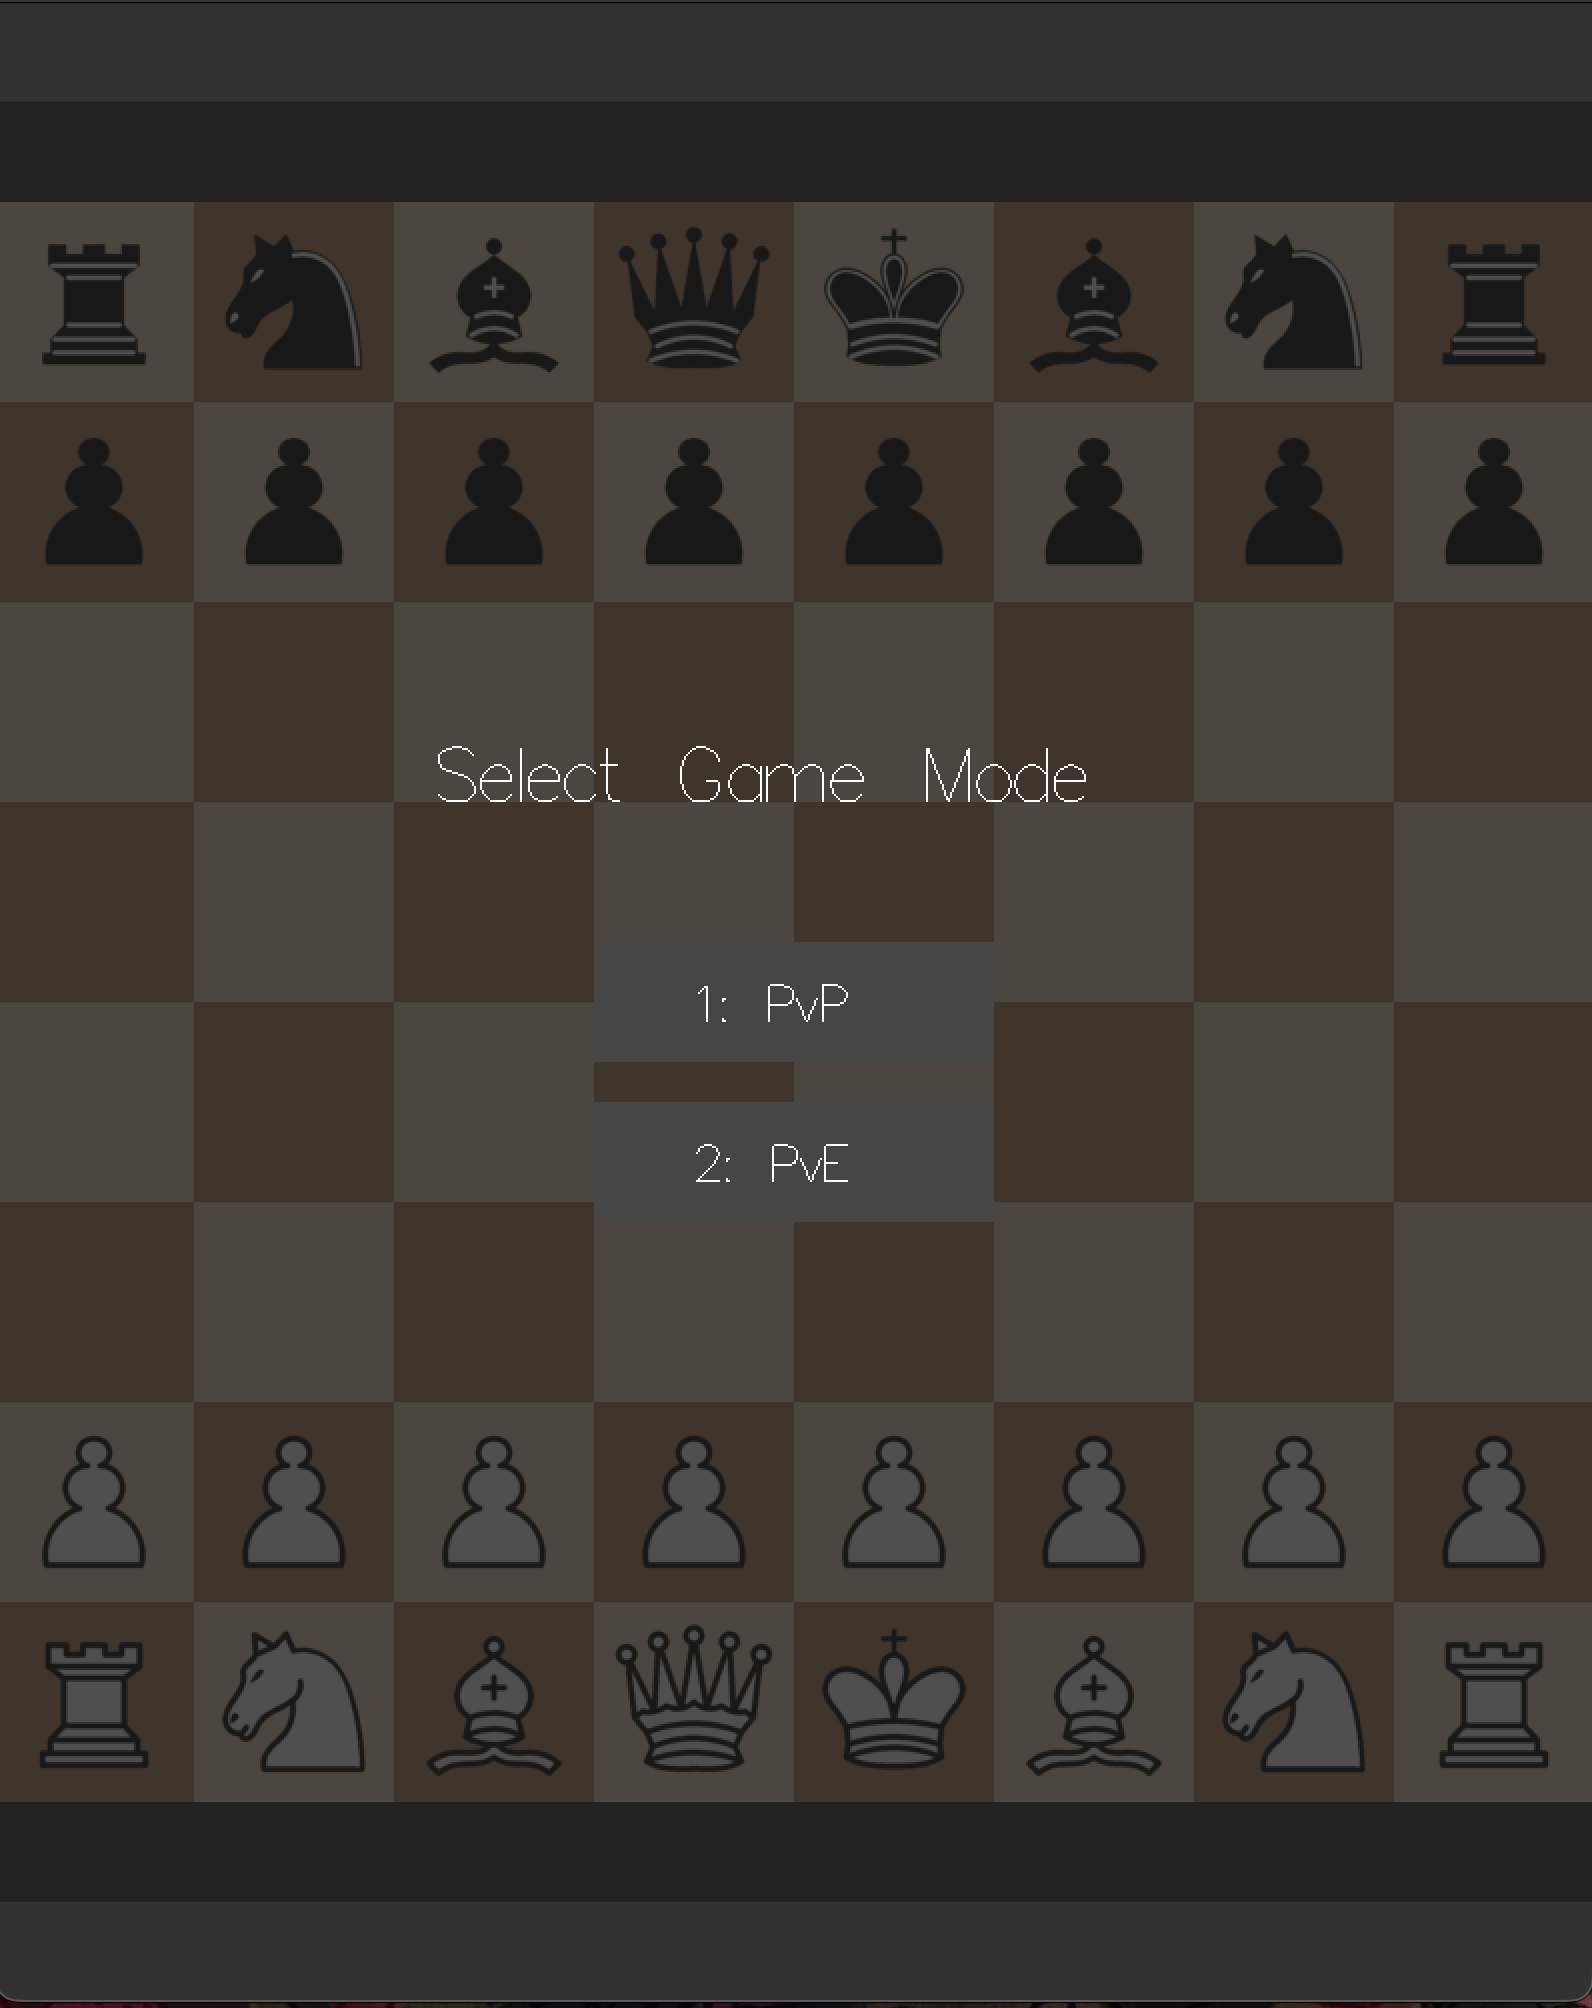
\includegraphics[width=0.8\textwidth]{./images/menu.png}
    \caption{Главное меню программы}
\end{figure}

Меню позволяет выбрать режим игры и запустить новую партию. В этом же месте выполняется выбор параметров одиночной игры, после чего программа переходит на экран доски и начинает партию с начальной расстановки фигур.

\begin{figure}[H]
    \centering
    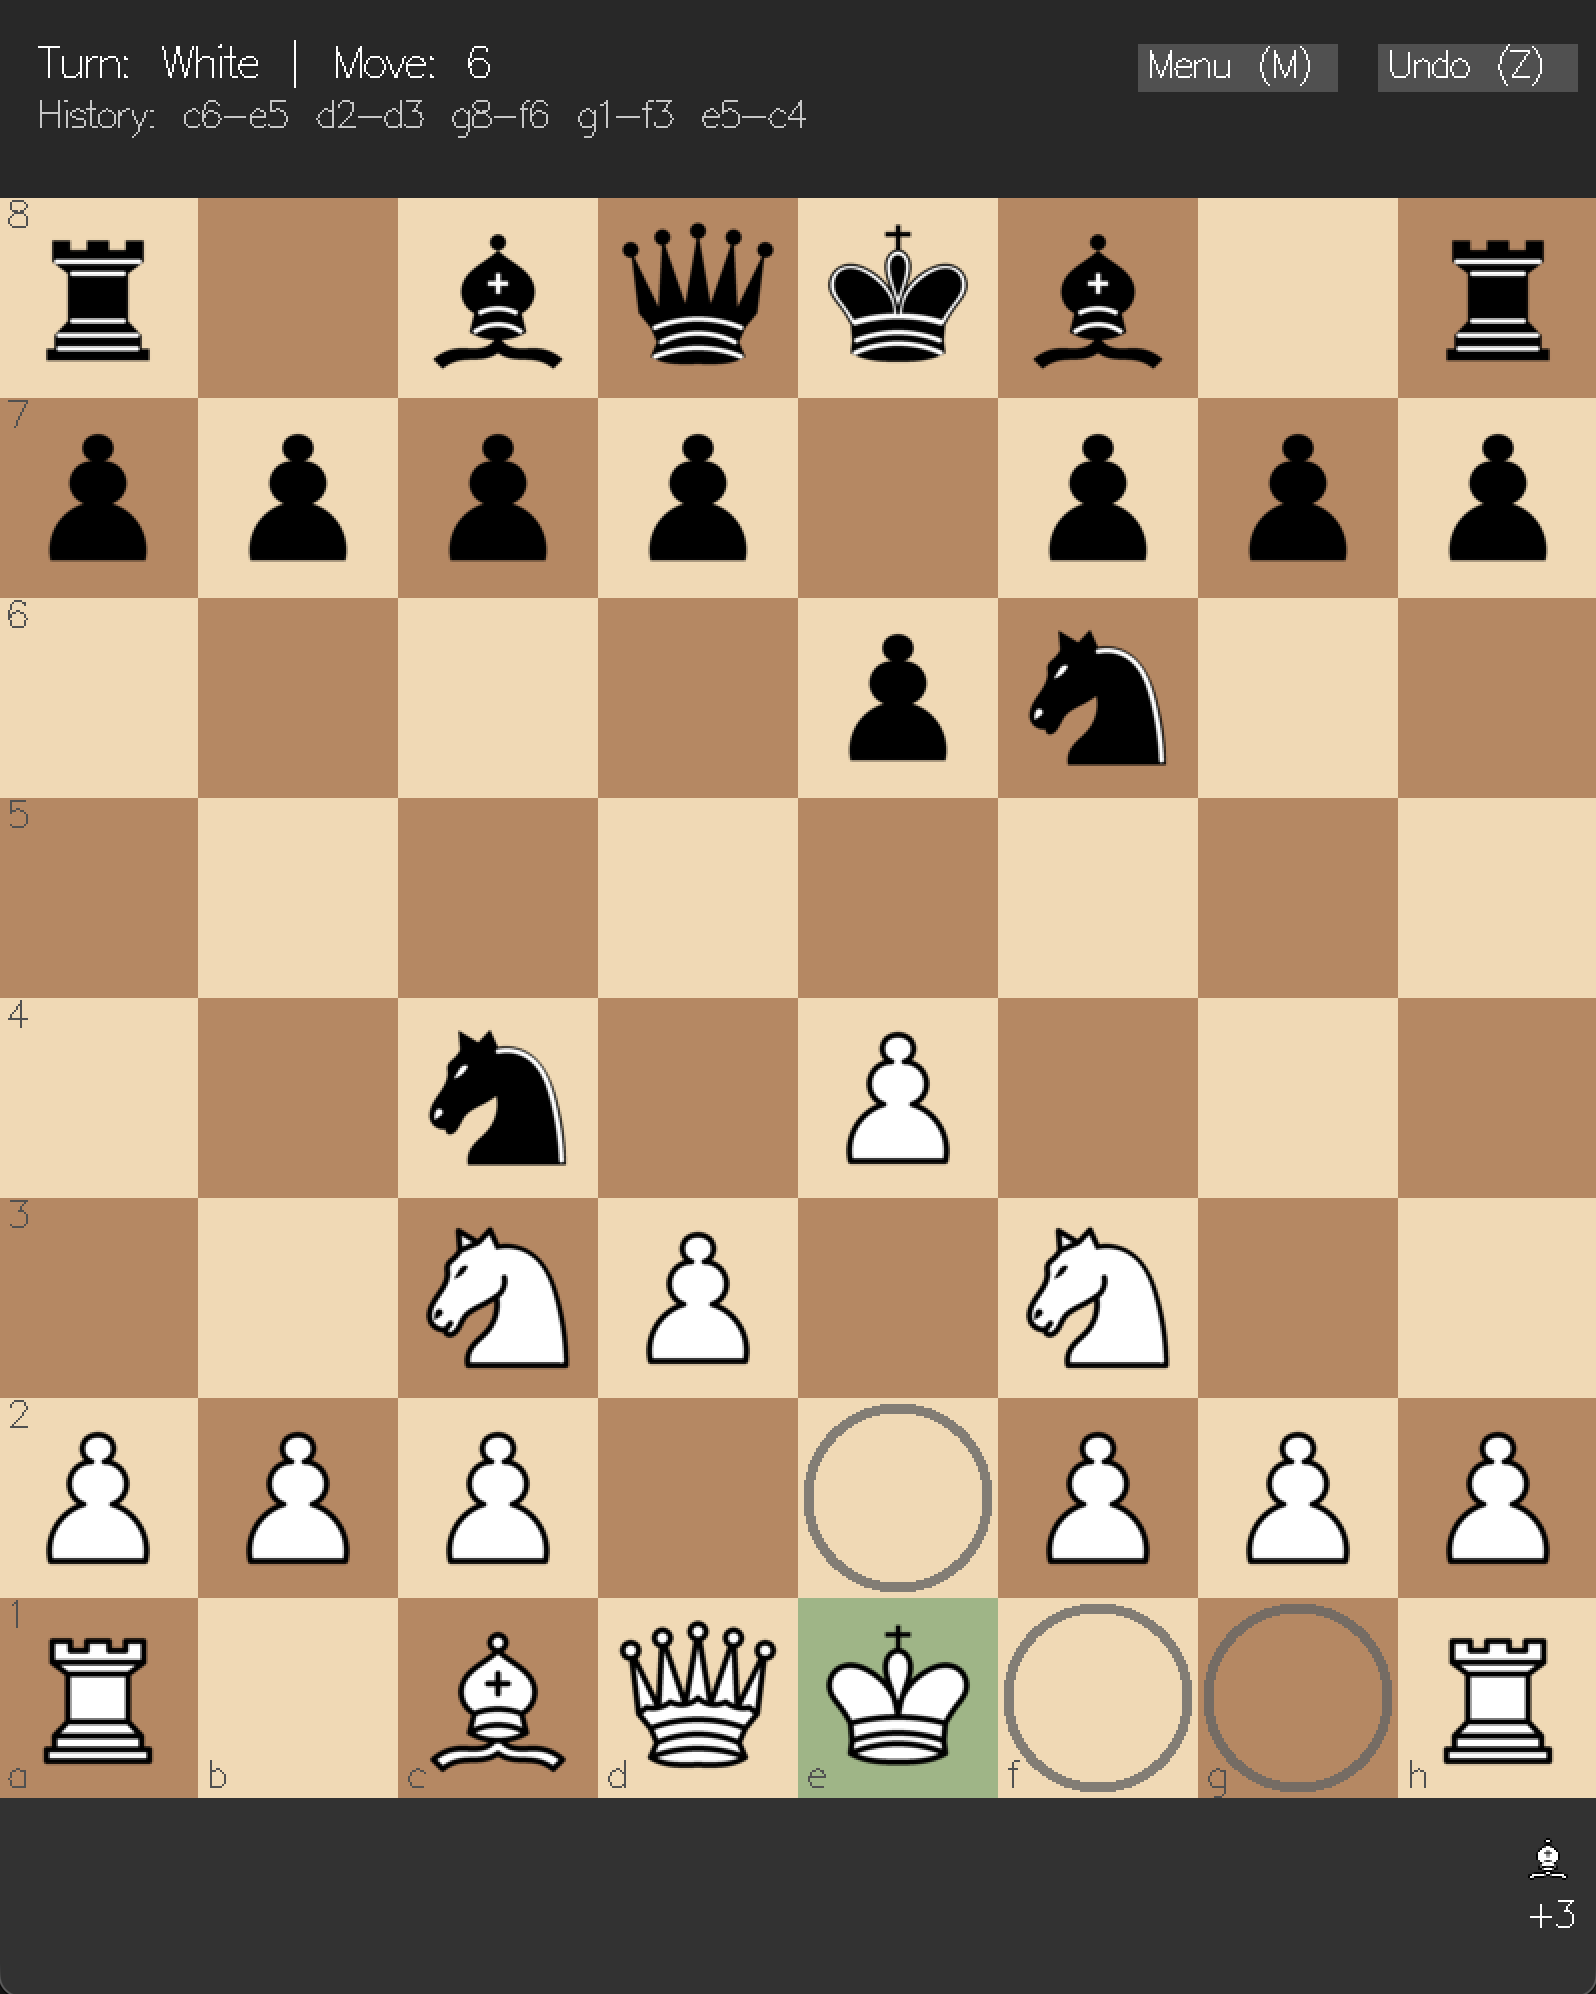
\includegraphics[width=0.8\textwidth]{./images/moves.png}
    \caption{Пример игрового процесса: разыграно несколько ходов}
\end{figure}

На данном примере (рис. 2) видно, как происходит выбор фигуры и подсветка допустимых клеток. После клика по своей фигуре программа строит список легальных ходов и показывает их на доске, поэтому игрок сразу понимает, какие перемещения разрешены правилами. После выполнения хода позиция на доске и строка истории обновляются синхронно, что помогает отслеживать ход партии.

\subsection{Работа программы}
Сначала пользователь кликает левой кнопкой мыши на свою фигуру, при этом клетка под ней загорается зеленым цветом. Клетки, на которые можно сделать шаг, отмечаются серыми кругами. При клике на нужную пустую клетку фигура мгновенно перемещается туда. Если включена игра против бота, компьютер делает свой ход, при этом время ожидания зависит от глубины поиска и вычислительной мощности компьютера. Завершенные шаги сразу отображаются в текстовой строке вверху.

\begin{figure}[H]
    \centering
    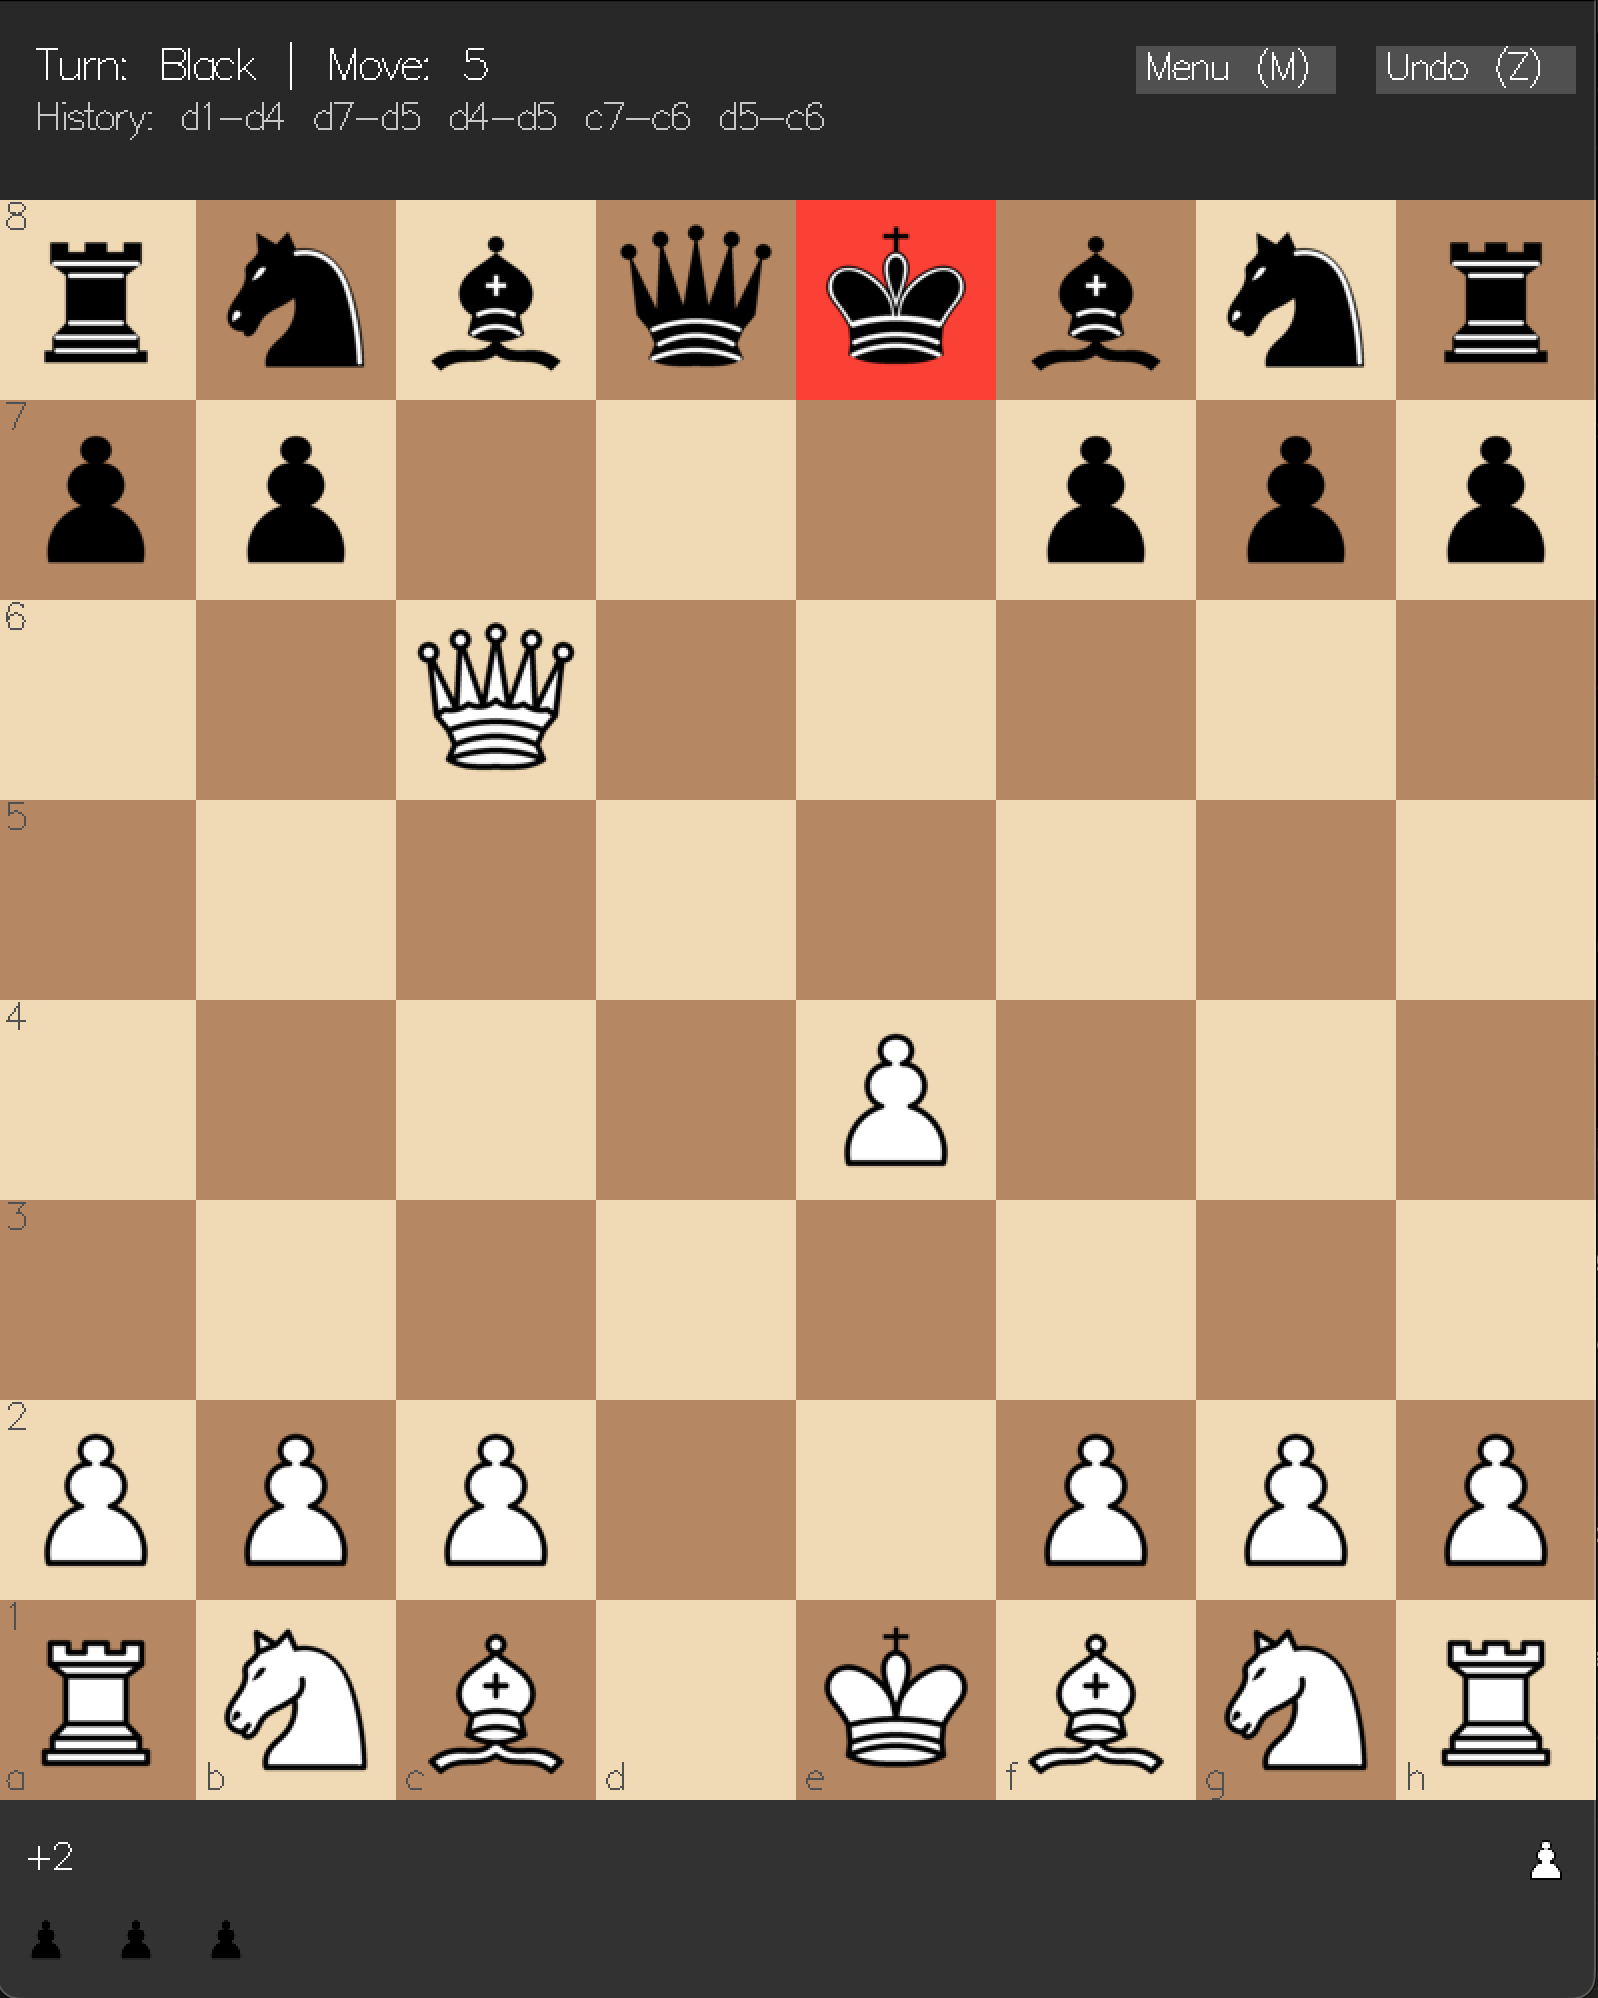
\includegraphics[width=0.8\textwidth]{./images/check.png}
    \caption{Ситуация шах: король находится под атакой}
\end{figure}

Когда возникает шах, программа вычисляет, атакована ли клетка короля фигурами противника. В этом состоянии разрешены только те ходы, которые убирают шах: уход короля, взятие атакующей фигуры или блокировка линии атаки (если это возможно). Любые попытки выполнить ход, оставляющий короля под ударом, автоматически отклоняются, поэтому пользователь не может нарушить правила.

\begin{figure}[H]
    \centering
    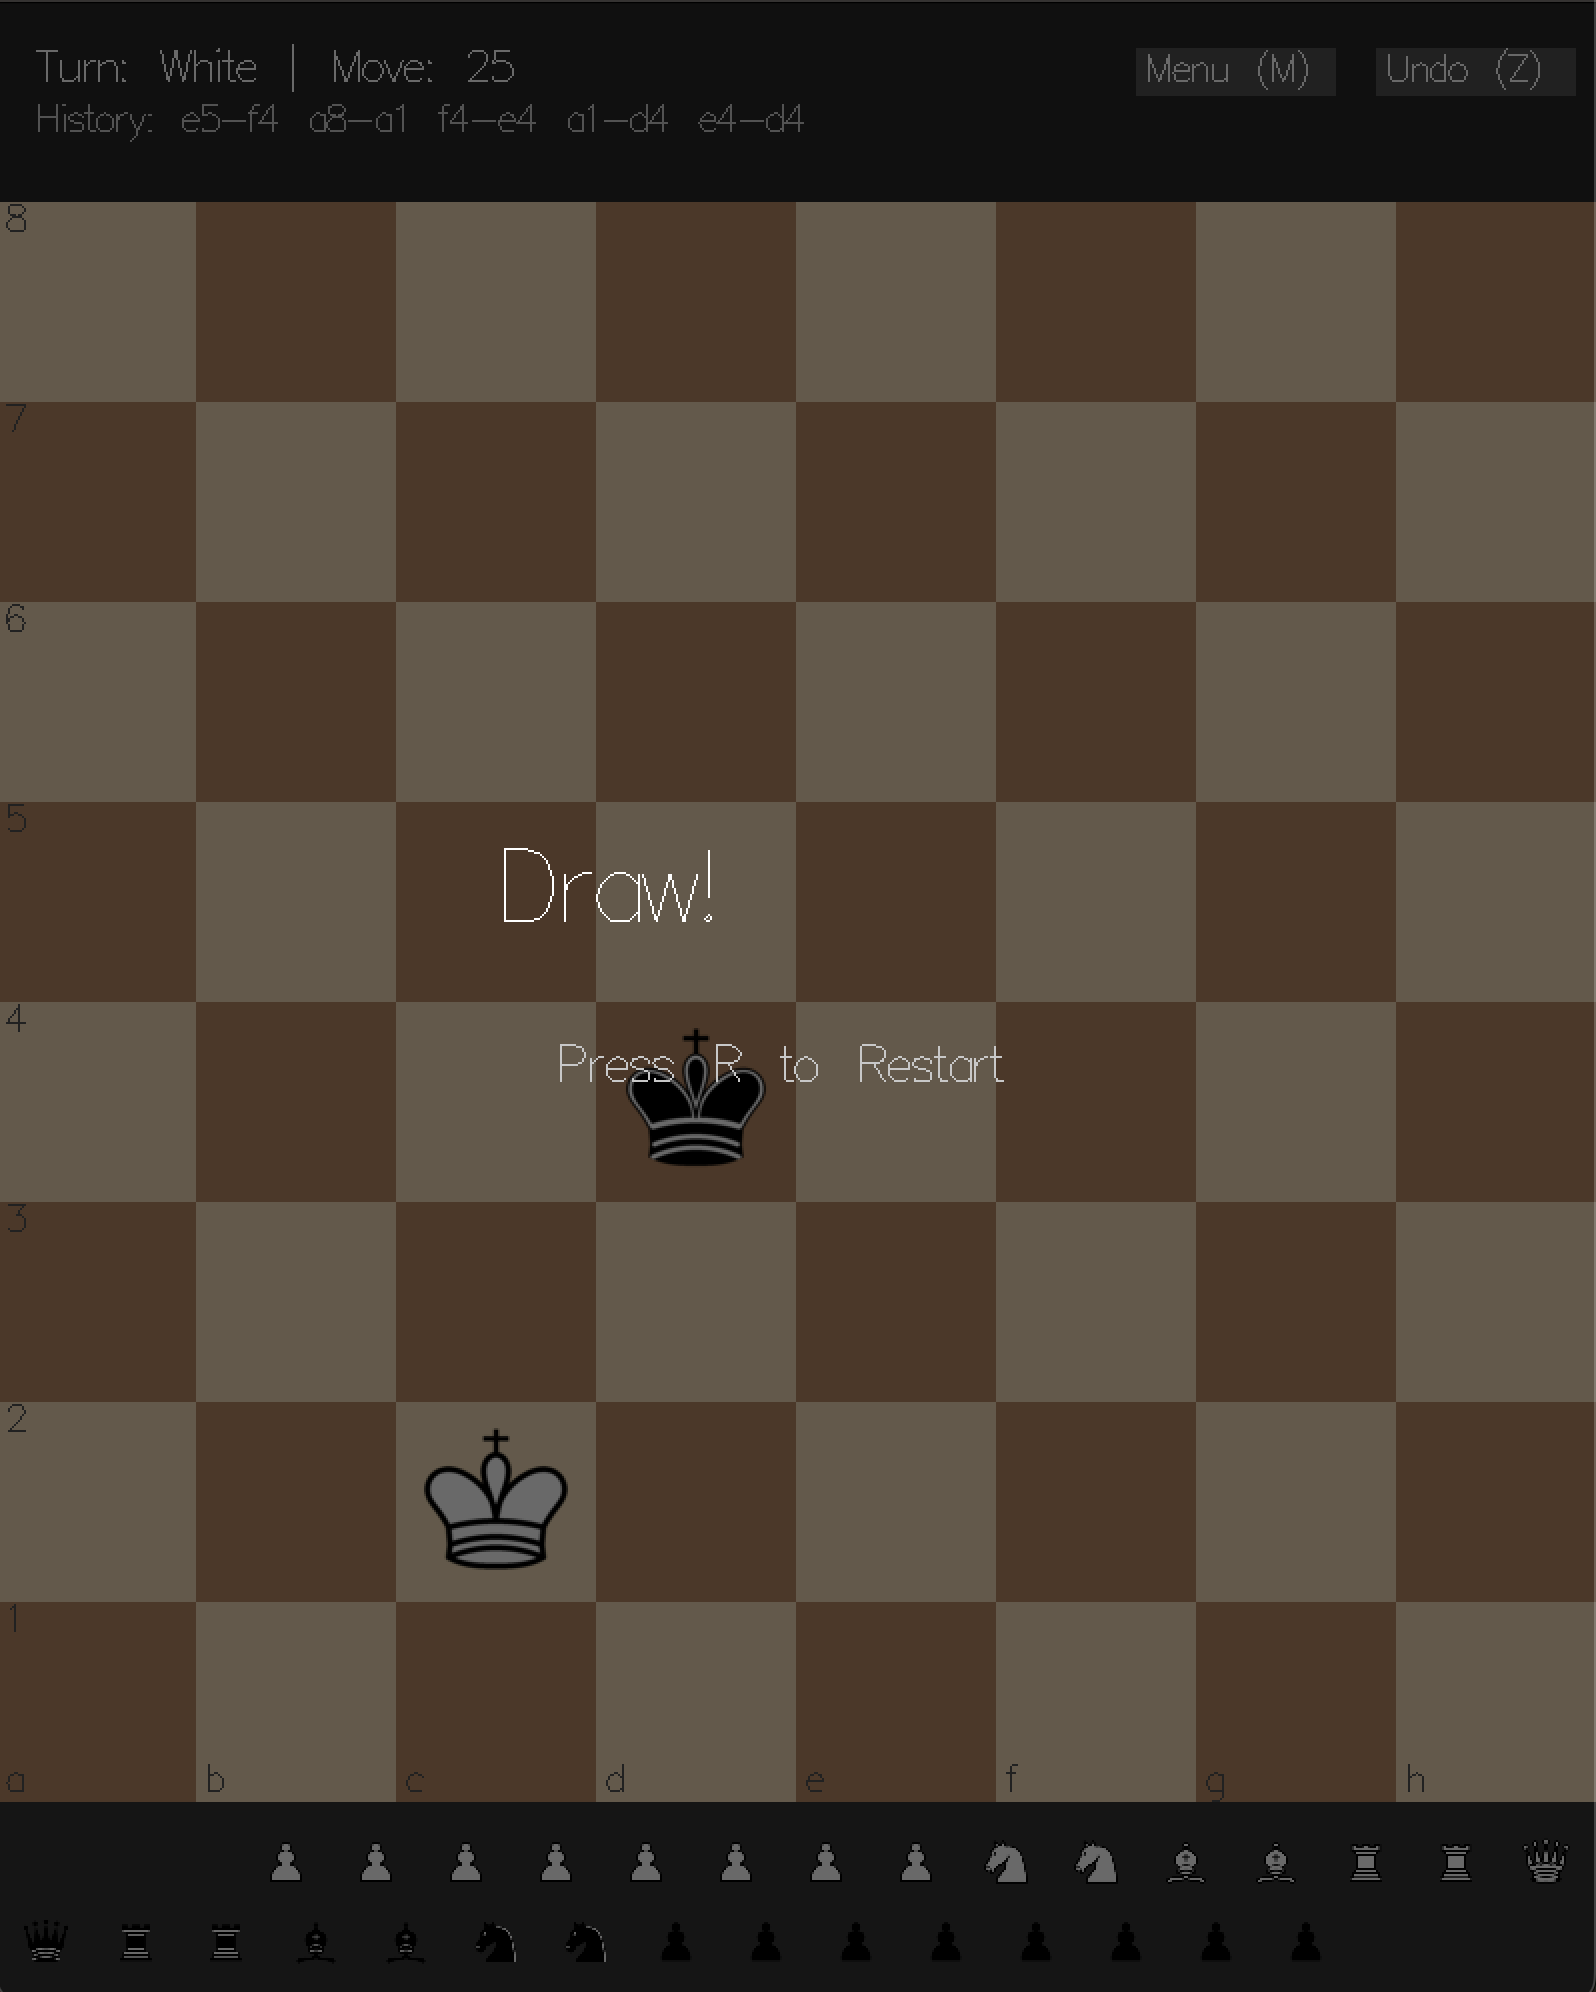
\includegraphics[width=0.8\textwidth]{./images/draw.png}
    \caption{Ситуация ничья: у игрока нет легальных ходов (пат) или зафиксировано завершение партии вничью}
\end{figure}

В ситуации ничьей программа проверяет, что у текущего игрока нет ни одного легального хода. Если при этом король не находится под шахом, фиксируется пат. После определения результата партия переводится в завершенное состояние, и дальнейшие ходы не выполняются, пока пользователь не начнет новую игру или не воспользуется перезапуском.

\subsection{Обработка ошибочных ситуаций}
Программа не позволяет человеку нарушить четкие правила шахмат. Если перемещение ставит собственного короля под прямой удар или король уже атакован, защита запретит двигать другие фигуры. Клик мышкой далеко за пределы кнопок или на пустую клетку просто игнорируется и никак не ломает игру.

\section{Отзывы}

\subsection{Отзыв: Андреев Илья Андреевич 324 АЯ}
Программа мне понравилась, авторы оставили указания с возможными действиями что очень помогло. Так же порадовал знакомый интерфейс и возможность игры против бота. 
Из предложений: ввести несколько уровней сложности бота
Минусы: предыдущий ход ии не показывается, ии играет один и тот же дебют

\subsection{Отзыв: Соловьев Ярослав Сергеевич 324 АЯ}
Как шахматы вполне нормально. Интерфейс очень простой. Отсутствует возможность выбора сложности бота. При попытке управлении через клавиатуру работает только с английской расскладкой.

\subsection{Отзыв: Ивановский Данила Сергеевич 324 АЯ}
Игра работает, интерфейс понятный. Бот играет часто однотипо. Было бы круто добавить возможность выбора сложности бота и отображение последнего хода.

\subsection{Отзыв: Коробов Евгений Алексеевич 324 АЯ}
Очень старался сломать программу. Но не получилось. Очень расстроился.

\subsection{Отзыв: Морозов Кирилл Олегович 317 ММП}
Игра работает корректно, багов  из разряда несуществующих ходов или типа того не обнаружил
Визуально, игра тоже сделана довольно хорошо
Есть пару моментов:
1) Не на весь экран почему-то отображалась игра. У меня их не видно истории ходов и другие статистики игры
2) Довольно часто компьютер после моего хода долго думает. Я снова думаю это связано с мощностями CPU (считааются сразу 5 следующих ходов, не самые лёгкие подсчёты, наверно). Больше 5 секунд ожидания.
3) Как раз к прошлому пункту: выбор сложности был бы не плох
4) добавить рандомайзер ходов
В остальном, очень крутой проект, я считаю (тестил только PvE режим, если что)

\subsection{Отзыв: Григорьев Александр Сергеевич 219}
Бот в целом неплох, но в дебюте играет очень пассивно, при этом развивая ферзя в начале, что считается неверной стратегией в общем случае.

Также могу сказать, что бот теряется в эндшпиле из-за маленькой глубины. Так как на этом этапе игры фигур мало, можно попробовать поднять глубину без сильной потери производительности

\subsection{Отзыв: Капитонов Станислав Сергеевич 219}
Бот неплох, дебют и миттельшпиль играет нормально, но в худшей позиции отказывается от троекратного повторения, тем самым допустив формированный мат

\section{Использование нейросетевых средств}
При проектировании архитектуры и написании кода для данного проекта диалоговые модели искусственного интеллекта применялись преимущественно в качестве интерактивного справочника. В самом начале работы над бэкендом (логическим движком) для консультации по правильному дизайну приложения нейросети был задан следующий промпт: 

\textit{«Я с товарищем собираемся написать шахматы на языке Хаскель. Это движок правил; типы данных: фигуры, цвет, клетка, доска, GameState; генерация псевдоходов для всех фигур; применение хода к состоянию; проверка шаха и фильтр легальности; спецправила: рокировка, en passant, превращение. Как должен быть организован проект? Хороша ли идея разбивать его на файлы-модули? На какие?»}

Опираясь на ответ ИИ как на структурный гайд, разработка была логично структурирована и поделена на смысловые файлы-модули (Board, Rules, Moves и др.), что сильно упростило параллельную работу соавторов. Выжимки из документации, предоставляемые нейросетью, помогли выбрать правильные абстракции для Haskell без необходимости долгого изучения тематических форумов.

Для реализации фронтенда нейросеть также выступала в роли справочника, но уже для уточнения особенностей функциональной библиотеки \texttt{gloss}. Задавались вопросы уточняющего характера: \textit{«Моя часть с Gloss... подскажи, как работает библиотека, как лучше организовать логику отрисовки и событий?»}. Поскольку библиотека использует специфический декларативный подход к событийному циклу, искусственный интеллект помог разобраться с тем, как транслировать чистые функции Haskell в непрерывное обновление окна. Он также подсказал удобные математические формулы для перевода курсора мыши (экранных пикселей) в индексы шахматной клетки. Это сработало как отличная выдержка из официальной документации и позволило быстро связать графический интерфейс с логическим движком.

Кроме того, нейросетевые средства помогли решить проблему дистрибуции игры. Был задан вопрос: \textit{«Можно ли собрать приложение в работающий .exe файл так, чтобы людям не нужно было скачивать Stack/cabal? Что такое .github/workflows/release.yml и как он должен выглядеть?»}. ИИ объяснил механику компиляции Haskell в независимый машинный код и предоставил готовый шаблон конфигурации для GitHub Actions. Благодаря этому теперь существуют готовые исполняемые программы (релизы) для Windows, macOS и Linux.

\section{Выводы}
В результате работы создана полная игра Шахматы. Реализован логичный графический интерфейс, проверка шахматных правил и умный компьютерный противник для одиночных партий. Проект показал пользу и удобство функционального подхода языка Haskell для реализации шахматной логики. Для проекта было собраны три релиза для разных операционных систем.
С проектом можно ознакомиться по ссылке:
\url{https://github.com/ovladisluvv/Haskell-Chess-2026}

\section{Литература}
\begin{enumerate}
    \item Hackage. Gloss: библиотека для простой 2D-графики и обработки событий. URL: \url{https://hackage.haskell.org/package/gloss}.
    \item The Haskell 2010 Report. Официальное описание языка Haskell. URL: \url{https://www.haskell.org/onlinereport/haskell2010/}.
    \item Chessprogramming Wiki. 8x8 Board: представление шахматной доски в виде массива. URL: \url{https://www.chessprogramming.org/8x8_Board}.
    \item Chessprogramming Wiki. Vector Attacks: вычисление атак дальнобойных фигур по направлениям. URL: \url{https://www.chessprogramming.org/Vector_Attacks} .
    \item Chessprogramming Wiki. Minimax: алгоритм поиска лучшего хода в играх. URL: \url{https://www.chessprogramming.org/Minimax}.
    \item Chessprogramming Wiki. Alpha-Beta: отсечение ветвей в минимаксе. URL: \url{https://www.chessprogramming.org/Alpha-Beta}.
    \item Chessprogramming Wiki. Simplified Evaluation Function: пример простой оценочной функции позиции. URL: \url{https://www.chessprogramming.org/Simplified_Evaluation_Function}.
    \item Chessprogramming Wiki. Mobility: учёт подвижности фигур в оценке позиции. URL: \url{https://www.chessprogramming.org/Mobility}.
\end{enumerate}


\end{document}